\documentclass[a4paper, 12pt]{report}
\usepackage{graphicx}

\begin{document}
	
\section{Electronics Modules Characterization}
\subsection{Coincidence Unit}
As the logic unit, the coincidence unit is a module used to make boolean operations between signals . The coincidence unit's imputs are logic pulses and the outputs are logic pulses if pulses appear at all imputs within a time interval (resolving time). In our experiment it is used(as the logic unit) to perform coincidences between signals.\\

The same approach used with the characterization of the logic unit can be applied to the coincidence unit.


The characterization setup is shown in Figure \ref{coinc_unit} and it is equivalent to the first set up for the logic unit . 

\begin{figure}[!h]
	\centering
	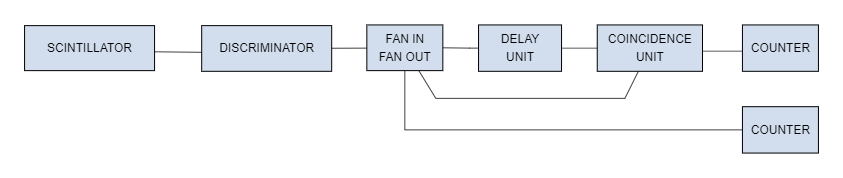
\includegraphics[width=\linewidth]{coinc_unit.png}
	\caption{Configuration employed during coincidence unit characterization}
	\label{coinc_unit}
\end{figure}


Also the fitting function(\eqref{eq:fermidirac}) and the way in which the errors are calculated are  always the same of the first characterization of the logic unit,thus the results can be shown directly. 


The estimated parameters are
\begin{eqnarray}
f_0 = 0.995 \pm 0.005\\
k = ( 20.936 \pm 9.790 ) \,  \si{ns^{-1}} \\
t_0 = ( 38.100 \pm 0.112 ) \,  \si{ns} .
\end{eqnarray}
and the covariance matrix is
\begin{equation}
\textrm{C}=\left(
\begin{array}{ccc}
     2.24 \cdot 10^{-5}  &  -1.39\cdot 10^{-2} &  -1.59 \cdot 10^{-4} \\
    -1.39 \cdot 10^{-2} &      95.84  &      0.98\\
    -1.59\cdot 10^{-4}  &       0.98   &    1.26\cdot 10^{-2} 
\end{array}
\right)
\end{equation}



The accordance between data and the model is excellent since $P_8\left(\chi^2\geq\chi_{obs}^2\right)=99.96\,\%$.
As in the  characterization of the logic unit it can be observed that  the counts fall quite sharply around a value of  delay and almost no counts are registered for delays greater than this.  
The value of this delay is almost \SI{38.1}{ns} and the time width of the coincidence unit obtained is: 

\begin{equation}
\delta_T = ( 0.191\pm 0.089 ) \, \si{ns}.
\end{equation}

The relative uncertainty obtained on $\delta_T$ is quite big $\left( \delta_{\delta_T} / \delta_T \sim 46.6 \%\right)$ since the decrease of the function is steep thus few data have been sampled in this region.   \\

\begin{figure}[!h]
	\centering
	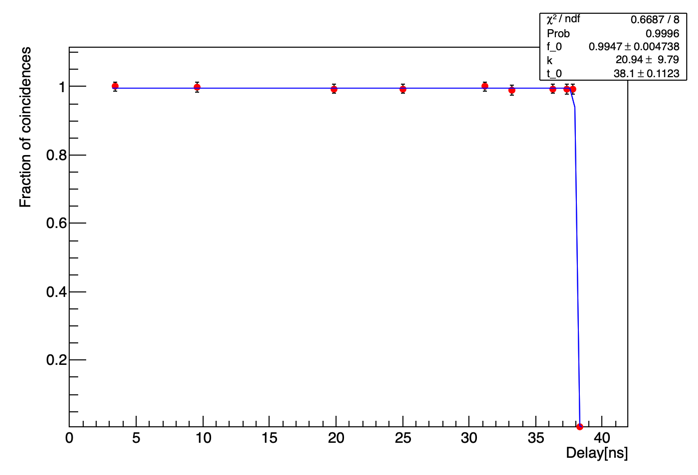
\includegraphics[width=\linewidth]{coinc_plot.png}
	\caption{Coincidence unit characterization}
	\label{coinc_plot}
\end{figure}



\end{document}